\documentclass[10pt]{beamer}
% Packages ----
\usepackage{amsmath}
\usepackage{amssymb}
\usepackage{booktabs}
\usepackage{xcolor}
\usepackage{bm}
\usepackage{graphicx}  
\usepackage{arydshln}
\usepackage{multicol}
\usepackage{multirow}
\usepackage{pbox}
\usepackage[style=nature, backend=biber]{biblatex}
% style=apa?
% \usepackage{enumitem} % doesnt work with beamer :(

\definecolor{codegreen}{rgb}{0,0.6,0}
\definecolor{codegray}{rgb}{0.5,0.5,0.5}
\definecolor{codepurple}{rgb}{0.58,0,0.82}
\definecolor{backcolour}{rgb}{0.95,0.95,0.92}
\definecolor{bostonuniversityred}{rgb}{0.8, 0.0, 0.0}

\newcommand{\eg}{e.g.\ }
\newcommand{\etc}{etc.\ }
\newcommand{\ie}{i.e.\ }
\newcommand{\textblue}[1]{\textcolor{blue}{#1}}
\newcommand{\textred}[1]{\textcolor{bostonuniversityred}{#1}}

% ----------------------------------------------------------
% Copying 00Preamble into this Presentation-specific one ---
% ----------------------------------------------------------

% Roman typefacing for design matrices
\newcommand{\X}{\mathrm{X}}
\newcommand{\Z}{\mathrm{Z}}
\newcommand{\D}{\mathrm{D}}

% Misc notation ----
\newcommand{\indep}{\perp\!\!\!\!\perp}   % Indendence, from https://tex.stackexchange.com/a/455701
\newcommand{\vech}{\text{vech}}           % vech text
\newcommand{\kth}{k^{\text{th}}}          % kth
\newcommand{\appx}{\overset{\text{appx.}}{\sim}} % Approximately follows
\renewcommand{\tt}[1]{\texttt{#1}}

% Brackets ----
\newcommand{\ls}{\!\left[}    % Left Square
\newcommand{\lb}{\!\left(}    % Left Bracket
\newcommand{\lbr}{\!\left\{}  % Left BRace
\newcommand{\rs}{\right]}   % Right Square
\newcommand{\rb}{\right)}   % Right Bracket
\newcommand{\rbr}{\right\}} % Right BRace

% Common Notation ----
\newcommand{\Y}{\bm{Y}_i}     % bold Y_i
\renewcommand{\b}{\bm{b}_i}   % bold b_i
\newcommand{\bb}{\bm{\beta}}   % bold \beta
\newcommand{\sek}{\sigma_{\varepsilon_k}^2} % sigma^2 eps with k subscript
\newcommand{\se}{\sigma_\varepsilon^2}      % sigma^2 eps
\newcommand{\K}{\bm{S}_i}      % K
\newcommand{\bz}{\bm{\zeta}}    % bold \zeta
\newcommand{\be}{\bm{\eta}_i}    % bold \eta_i
\newcommand{\li}{\lambda_i}    % \lambda
\newcommand{\lo}{\lambda_0}    % \lambda_0, baseline hazard
\newcommand{\bg}{\bm{\gamma}}  % bold \gamma
\newcommand{\vD}{\vech\lb\D\rb} % vech(D)
\DeclareMathOperator{\Exp}{\mathbb{E}}
\newcommand{\Expi}[1]{\mathbb{E}_i\ls#1\rs}
\newcommand{\Var}{\mathrm{Var}}
\newcommand{\torm}[2]{#1^{(\mathrm{#2})}}

% Summations and products ----          (sum for {x} = 1, ... ,{y})
\newcommand{\Si}{\sum_{i=1}^n}                   %i             n 
\newcommand{\SiN}{\sum_{i=1}^N}                  %i             N 
\renewcommand{\Pi}{\prod_{i=1}^n}   % (Product)   i             n
\newcommand{\Sj}{\sum_{j=1}^{m_i}}               %j             m_i
\newcommand{\Sk}{\sum_{k=1}^K}                   %k             K
\newcommand{\Sl}{\sum_{l=1}^\varrho}             %l             \rho
\newcommand{\dsum}{\bigoplus_{k=1}^K} % Direct sum

% Simulation stuff ------
\newcommand{\Keta}{\bm{S}^\top\bz} % K*eta
\newcommand{\intzt}{\int_0^t}   % int 0->t
\newcommand{\simsurvofrac}{\frac{1}{Q+\alpha}} % outside fraction
\newcommand{\simsurvlog}[1]{1+\frac{(Q+\alpha)#1}{\nu\exp\lbr P\rbr}}


% Densities ----
% Short form: \sf<outcome> - f(<outcome>|\Omega)
\newcommand{\sfY}{f\lb\Y|\b;\bO\rb}           % short longit
\newcommand{\sfT}{f\lb T_i,\Delta_i|\b;\bO\rb} % short survival
\newcommand{\sfRE}{f\lb\b|\bO\rb}             % short RE
\newcommand{\bY}{f\lb\b|\Y;\bO\rb}     % b|y
% Full form: \ff<outcome> - f(<outcome>|<everything it's conditional upon; params)
\newcommand{\ffY}{f(\Y|\mathrm{X}_i,\b;\bb,\sigma^2_{\varepsilon_1},\dots,\sigma^2_{\varepsilon_K})}     %longit
\newcommand{\ffT}{f(T_i,\Delta_i|\K,\b;\bz,\bg)} %survival
\newcommand{\ffRE}{f(\b|\mathrm{D})} %REs
\newcommand{\condb}{f\lb\b|T_i, \Delta_i, \Y; \bO\rb}
\newcommand{\condbh}{f\big(\b|T_i, \Delta_i, \Y; \hbO\big)}
\newcommand{\argmax}[1]{\underset{#1}{\rm{argmax}}}
\newcommand{\cS}{\mathcal{S}_i}


% Parameter vector ----
\newcommand{\bO}{\bm{\mathrm{\Omega}}}       % non-hat notation
\newcommand{\paramvec}{\bb,\sigma^2_{\varepsilon_1},\dots,\sigma^2_{\varepsilon_K},\be,\bg,\vech(\mathrm{D})} 
\newcommand{\hbO}{\hat{\bm{\Omega}}}% hat notation
\newcommand{\hparamvec}{\hat{\bb},\hat{\sigma}^2_{\varepsilon_1},\dots,\hat{\sigma}^2_{\varepsilon_K},
                        \hat{\be},\hat{\bg},\vech(\hat{D})}
                        
% hat notation ----
\newcommand{\hb}{\hat{\bm{b}}_i}     % bold b_i hat
\newcommand{\hS}{\hat{\Sigma}_i}     %  \Sigma_i hat
\newcommand{\hbb}{\hat{\bb}}         % hat bold beta
% Sigma_i
\newcommand{\pt}{\partial} 
\newcommand{\compdata}{f\big(\b,T_i,\Delta_i,\Y;\hbO\big)} %Complete data|parameters
\newcommand{\Napprox}{N\big(\hb,\hS\big)}

% Parameter Updates
\newcommand{\tobm}[1]{#1^{(m)}}
\newcommand{\tobmp}[1]{#1^{(m+1)}}
\newcommand{\tExpi}[1]{\tilde{\mathbb{E}}_i\ls#1\rs}
\newcommand{\elli}[1]{\ell_i\lb#1\rb}
\newcommand{\unsetp}[1]{\underset{#1}{\propto}}
\newcommand{\crossprod}[2]{#1^\top#2}
\newcommand{\tcrossprod}[1]{#1#1^\top}
\newcommand{\bmu}{\bm{\mu}_i}
\newcommand{\hbmu}{\hat{\bm{\mu}}_i}
\newcommand{\Amat}{\mathrm{A}_i}
\newcommand{\btau}{\bm{\tau}_i}
\newcommand{\diag}[1]{\mathrm{diag}\lb#1\rb}
\newcommand{\dXdY}[2]{\frac{\pt#1}{\pt#2}}
\newcommand{\dXdYdY}[2]{\frac{\pt#1}{\pt#2\pt#2^\top}}

% Justifications
\newcommand{\bOT}{\bO^{(\mathrm{TRUE})}}
\newcommand{\TRUE}[1]{#1^{(\mathrm{TRUE})}}
\newcommand{\margfull}{f\lb\bm{b}_i|T_i,\Delta_i,\bm{Y}_i;\bO^{(\rm{TRUE})}\rb}
\newcommand{\postb}{f\big(\b|\mathcal{D}_i;\bOT\big)}
\newcommand{\tb}{\tilde{\bm{b}}_i}
\newcommand{\tS}{\tilde{\Sigma}_i}
\newcommand{\Rapprox}{N\big(\tb,\tS\big)}

% GLMMs
\newcommand{\bphi}{\bm{\varphi}_i}
\newcommand{\bs}{\bm{\sigma}}
\newcommand{\lgam}[1]{\log\Gamma\lb#1\rb}
\newcommand{\gam}[1]{\Gamma(#1)}
\newcommand{\linpRHS}{\X_i\bb+\Z_i\b}
\newcommand{\linp}{\bm{\eta}_i}
\newcommand{\linpk}{\bm{\eta}_{ik}}
\newcommand{\W}{\mathrm{W}_i}
\newcommand{\boneT}{\bm{1}^\top}
\newcommand{\bone}{\bm{1}}
\newcommand{\dotlinp}{\dot{\bm{\eta}}_i}
\newcommand{\ddotlinp}{\ddot{\bm{\eta}}_i}

% Dynpreds
\newcommand{\subrm}[2]{#1_{\mathrm{#2}}}
\newcommand{\Tstart}{\subrm{T}{start}}
\newcommand{\nalive}{\subrm{n}{alive}}
\newcommand{\Twindow}{(\Tstart,\Tstart+\delta]}
\newcommand{\cL}{\mathcal{L}}
\newcommand{\hpw}{\hat{\pi}_i\lb w\rb}
\newcommand{\idx}[1]{\tt{id}\ #1\ }
\newcommand{\auc}[1]{\mathrm{AUC}_{#1}}
\newcommand{\wPE}{\widehat{\mathrm{PE}}}
% Theme -----------------------------
\usetheme{default}
\usecolortheme{beaver}

% Title page ------------------------
\title{Fast fitting for joint models of survival and multivariate longitudinal data} 
\author{James Murray}
\date{PhD Viva, $1^{\mathrm{st}}$ May 2024}
\titlegraphic{
\includegraphics[width = 0.5\textwidth]{logo.jpg}}
 
% Customise captions ---------------
\setbeamerfont{caption}{size=\tiny}
\def\vfilll{\vskip 0pt plus 1filll minus 0pt }
% Bib
\addbibresource{refs.bib}

% Start presentation
\begin{document}

\begin{frame}
    \vfilll
    \titlepage
    \vfilll
    \small
    Supervisor: Dr.\ Pete Philipson
\end{frame}

% Outline
\begin{frame}{Outline}
A whistle-stop tour...

\begin{itemize}
    \item Introduction: Joint models, motivation
    \vspace{2mm}
    \item ``Classic'' multivariate joint models
    \vspace{2mm}
    \item \textblue{An approximate EM algorithm}
    \vspace{2mm}
    \item \textblue{Flexible joint models}
    \vspace{2mm}
    \item Justification for approximation used
    \vspace{2mm}
    \item Post-hoc analysis; prediction
    \vspace{2mm}
    \item Application to PBC
    \vspace{2mm}
    \item Discussion; future avenues for research
\end{itemize}
    
\end{frame}

% Introduction
\section{Introduction}
\begin{frame}{Background: Joint modelling}
    Initially arose as a solution to answer analytical challenges in HIV/AIDS research.\\

    \vspace*{5mm}

    Predated by both na\"{i}ve and ``two-stage'' methods, both of which don't provide wholly efficient use of available data.\\

    \vspace*{5mm}

    Joint models as they appear in the thesis first given in Wulfsohn \& Tsiatis (1997) \cite{Wulfsohn97}.\\

    \vspace*{5mm}
    Joint models typically consists of (at least) two sub-models linked together by shared random effects.\\
    Models for the longitudinal and survival parts are `joined' together.
\end{frame}

\begin{frame}{Evolution}
    Since their first (basic) formal presentation in Wulfsohn \& Tsiatis, joint models have been expanded and extended in numerous ways:
    \begin{itemize}
        \item Multivariate case:\\
        $\hookrightarrow$ Measuring association of $\ge2$ longitudinal responses with survival, accounting for correlations.
        \item Random effects:\\
        $\hookrightarrow$ More complex (\eg splines); more longitudinal sub-models
        \item Alternative sub-models:\\
        $\hookrightarrow$ Replacing the Cox PH or the longitudinal model by something more appropriate.
    \end{itemize}
    \vspace*{5mm}
    Each serve to increase complexity in the joint model and introduce issues in standard fitting routines; reflected in lack-of software for many cases.
\end{frame}

\section{Motivation: PBC}
\begin{frame}{Motivating data}
One popular application is to primary biliary cirrhosis (PBC).
\vspace*{5mm}
\begin{figure}
    \centering
    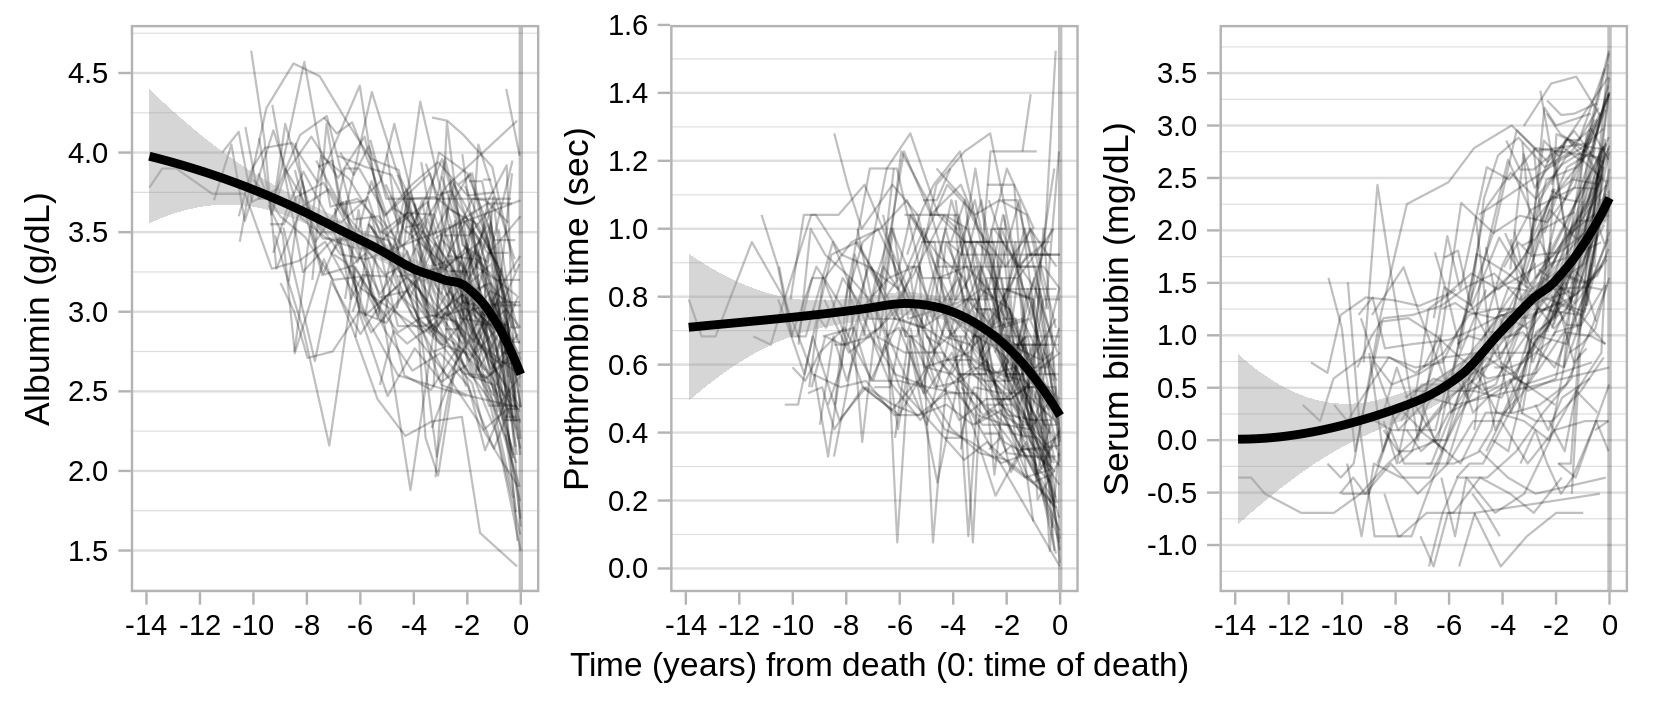
\includegraphics[width=0.975\textwidth]{Figures_Chapter1/PBCtrajectories.png}
    \caption{Patient trajectories for three biomarkers measured during Mayo Clinic trial \cite{PBCarticle}.}
    \label{fig:pbc-trajectories}
\end{figure}
    
\end{frame}

\begin{frame}{Motivating data}
One popular application is to primary biliary cirrhosis (PBC).\\
\vspace*{5mm}
A joint analysis allows researchers to \textit{simultaneously} answer:

\begin{enumerate}
    \item How do these biomarkers evolve through time and differ in terms of covariates collected at baseline (\eg drug allocation, sex, age)?
    \item How does the hazard of interest evolve through time an differ in terms of covariates collected at baseline?
    \item How is the hazard affected by underlying biomarker values?
\end{enumerate}
    
\end{frame}

\section{Classic Joint Models}
\begin{frame}{Joint modelling framework: Notation}
For each $i=1,\ldots,n$ we observe the $\kth, k=1,\ldots,K$ longitudinal response $\Y{_k}=\lb y_{i1k},\ldots,y_{i{m_i}k}\rb^\top$.\\

\vspace*{2mm}

Event time $T_i=\min\lb T_i^*, C_i\rb$ and $\Delta_i=1$ if $T_i^*<C_i$ and $\Delta_i=0$ otherwise.\\

\vspace*{2mm}

Form a joint model by inducing an association between the $K$ longitudinal trajectories and the hazard $\lambda_i$:
  \begin{equation*}
    \begin{aligned}
    \begin{cases}
      \Y{_k} &\!\!\!\!\!\!\!\!\!\!\!\!\!\!= \X_{ik}\lb t\rb\bb_{k} + \Z_{ik}\lb t\rb\textblue{\b{_k}} + \bm{\varepsilon}_{ik}\\
      \ \ \ \ \ \ \ \b{_k} &\!\!\!\!\!\sim N_{q_k}\lb 0, \mathrm{D}_k\rb, \quad \bm{\varepsilon}_{ik}\sim N\lb0, \sigma^2_{\varepsilon_k}\rb,\quad \b{_k}\indep\bm{\varepsilon}_{ik}\\
      \lambda_i(t)&\!\!\!\!\!\!\!\!\!\!\!\!\!\!=\lambda_0(t)\exp\lbr\bm{S}_i^\top\bm{\zeta} + \Sk\textblue{\gamma_k\bm{W}_k(t)^\top\b{_k}}\rbr.  
    \end{cases}
    \end{aligned}
  \label{eq:methods-lmm}
  \end{equation*}
  where the association parameter \textblue{$\gamma_k$} captures association between  $\b{_k}$ on the hazard.
    
\end{frame}

\begin{frame}{Estimation}
    Want to estimate the following parameters:
    \begin{align*}
    \bO=\lb\vD^\top,\bb^\top,\sigma^2_{\varepsilon_1},\ldots,\sigma^2_{\varepsilon_K},\bg^\top,\bz^\top\rb^\top
    \end{align*}
    which we do my maximising the observed data likelihood via an EM algorithm.\\
    \vspace{2mm}
    \textbf{E-step} at iteration $(m+1)$:
    \begin{equation*}
    \begin{aligned}
      \Si \Exp_i\!\bigg[&\log f\lb\Y|\b;\bO^{(m)}\rb + \log f\lb T_i,\Delta_i|\b;\bO^{(m)}\rb+\log f\lb\b|\bO^{(m)}\rb\bigg].
    \end{aligned}
  \label{eq:methods-E-step}
  \end{equation*}
  calculated against $f\lb\b|T_i,\Delta_i,\Y;\bO^{(m)}\rb$\\
  \vspace{2mm}
  \textbf{M-step}: Formed by maximising $n$ \textit{sets} of conditional expectations.
    
\end{frame}

\begin{frame}{Estimation}
    All required expectations necessary in each EM iteration are of form:
    \begin{align*}
        \Exp_i\ls g\lb\b\rb|T_i,\Delta_i,\Y;\bO\rs=
        \frac{\int_{-\infty}^\infty g\lb\b\rb f\lb T_i,\Delta_i|\b;\bO\rb f\lb\b|\Y;\bO\rb d\b}{\int_{-\infty}^\infty f\lb T_i,\Delta_i|\b;\bO\rb f\lb\b|\Y;\bO\rb d\b}
    \end{align*}
    where $f\lb\b|\Y;\bO\rb$ enjoys tractable form under MVN $\Y$ \cite{Wulfsohn97, Hickey2018}.\\
    \vspace{5mm}
    Numerical methods used to evaluate these multi-dimensional integrals.\\
    \vspace{5mm}
    Main source of computation burden -- especially with \textit{more complex} model specifications -- potentially precluding uptake.
\end{frame}

\section{Approximate EM}
\begin{frame}{An approximate EM algorithm}
Key issue is that $\condb$ is potentially high dimensioned.\\

\vspace{5mm}

Bernhardt \textit{et al}.\ (2015) \cite{Bernhardt15} propose
\begin{align*}
    \b|T_i,\Delta_i,\Y;\bO^{(m)}\appx N\big(\hb,\hS\big)
\end{align*}
Thereby allowing all requisite expectations $\Exp_i\ls g\lb\b\rb|T_i,\Delta_i,\Y;\bO^{(m)}\rs$ to be taken against a univariate normal distribution.\\

\vspace{5mm}
Originally proposed in context of a multivariate joint model with a logistic regression model in place of the Cox PH.\\

\vspace{5mm}

Novel contribution then the extension to more `traditional' joint models.
\end{frame}

\begin{frame}{An approximate EM algorithm}

\begin{enumerate}
    \item Obtain initial conditions $\bO^{(0)}$
    \vspace{2mm}
    \item For \textit{any} iteration $(m+1)$:
    \begin{enumerate}
        \item Obtain $\hb$ and $\hS$ by maximising $\log f\lb\b,T_i,\Delta_i,\Y;\bO^{(m)}\rb$ using \tt{optim}
        \item Use the normal approximation to update the parameter vector $\bO^{(m)}\rightarrow\bO^{(m+1)}$.
    \end{enumerate}
    \vspace{2mm}
    \item Check for convergence
    \vspace{2mm}
    \item Repeat steps 2.\ and 3.\ for at least four iterations, then exit when 3.\ satisfied.
\end{enumerate}
    
\end{frame}

\begin{frame}{An approximate EM algorithm: Results}

Many simulation studies carried out to ascertain performance.

\begin{itemize}
    \item Sample size;
    \item Length of follow-up;
    \item Number of responses \etc
\end{itemize}
All studies tabulated and presented graphically.

\vspace{3mm}

Good performance across all simulations considered as well as sensitivity analyses.\\

\vspace{3mm}

Compared with \tt{joineRML} \cite{Hickey2018} where results were very similar.\\

\vspace{3mm}

Non-exponential increase in computation time observed.
    
\end{frame}

\section{Flexible joint models}
\begin{frame}{Flexible specifications}
    Gaussian assumption ubiquitous but may not best represent data\\

    \vspace{1mm}

    $\hookrightarrow$ Important to accommodate (range of) response types\\

    \vspace{5mm}

    If $\Y|\b$ assumed normal, $f\lb\b|T_i,\Delta_i,\Y;\bO\rb$ is tractable\\

    \vspace{5mm}

    Issues arise when this assumption isn't met and the above thereby not tractable.\\
    \vspace{1mm}
    $\hookrightarrow$ Led to predominantly Bayesian approaches to inference in the literature.\\

    \vspace{5mm}

    Promising then that the normal approximation eschews consideration of $\Y|\b$, instead collapsing down $f\lb\b|T_i,\Delta_i,\Y;\bO\rb$ to $\Napprox$
    
\end{frame}

\begin{frame}{Flexible specifications}
    Considered six exponential families for GLMMs:
    \begin{table}[h]
        \centering
        \begin{tabular}{ccc}
            (Gaussian) & Poisson & Binomial \\
            Negative binomial & Generalised Poisson & Gamma
        \end{tabular}
    \end{table}
    \vspace{3.75mm}
    Estimation of $\bO$ (potentially with dispersion parameters) via approximate EM algorithm.\\

    \vspace{5mm}

    Simulations chosen to reflect possible modelling scenarios and investigate performance in `non-standard' scenarios.\\
    \vspace{1mm}
    $\hookrightarrow$ 
    Performance good overall, worst performance for binomial.\\
    \vspace{1mm}
    $\hookrightarrow$
    No obvious deterioration in performance in terms of estimation or computation time
    
\end{frame}

\begin{frame}{Justification for normal approximation}
    Approximating $\b|T_i,\Delta_i,\Y;\bO\sim\Napprox$ throughout\\
    
    \vspace{1mm}
    
    $\hookrightarrow$ Good idea to investigate and justify this!\\
    
    \vspace{5mm}
    
    Compared the `true' posterior for given scenario $f\big(\b|T_i,\Delta_i,\Y;\bOT\big)$\\to $\Napprox$ visually and via `coverage' of the approximation.\\

    \vspace{5mm}

    Overall the approximation does appear reasonable, but evidence to suggest it's over-confident (\ie $\hS$ overestimated slightly).\\

    \vspace{5mm}

    Additionally investigated differences in $\Napprox$ when $\hb, \hS$ obtained with/out $\lbr T_i, \Delta_i\rbr$.\\

    \vspace{5mm}

    Non-exhaustive, but allow us to get a handle on $\Napprox$.
    
\end{frame}

\section{Post Hocs}
\begin{frame}{Model diagnostics \& prediction}
    In lieu of a `joint' residual, consider one for each sub-model.\\

    \vspace{5mm}

    Hypothesis testing: Wald tests, AIC, BIC.\\

    \vspace{5mm}

    Dynamic predictions \cite{Rizopoulos2011}, future survival to time $u$ given data up-to $t$:
    \vspace{1mm}
    \begin{itemize}
        \item Estimation of $\pi_i\lb u|t\rb$ involves $\b|T_i^*>t,\Y{_1}\lb t\rb,\ldots,\Y{_K}\lb t\rb; \hbO$.\\Either by empirical Bayes or Monte Carlo scheme.
        \vspace{1mm}
        \item Ascertain predictive performance across `windows' $w=(\Tstart,h]$\\
        $\uparrow\Tstart\implies$ more information available$\implies$ better performance?
        \vspace{1mm}
        \item Set out performance measures $\mathrm{AUC}\lb w\rb$ and $\widehat{\mathrm{PE}}\lb w\rb$
        \vspace{1mm}
        \item Comparing nested models
        \vspace{1mm}
        \item Correcting for optimism in these estimates.
    \end{itemize}

    \vspace{5mm}

    Basically, setting out metrics to use in an application...
    
\end{frame}

\section{Application}
\begin{frame}{Application: Primary biliary cirrhosis}
    Aim was to present a start-to-finish model building process utilising approximate EM for joint model portion:
    \vspace{1mm}
    \begin{itemize}
        \item Exploratory analysis and data description:\\
        Clinical outcome, baseline covariates, candidate longitudinal markers.
        \vspace{0.5mm}
        \item Survival sub-model selection 
        \vspace{0.5mm}
        \item Longitudinal sub-model selection for each biomarker:\\
        Combinations of fixed effects, time specification
        \vspace{0.5mm}
        \item Strength of \textit{univariate} associations
        \vspace{0.5mm}
        \item `Groups' of markers defining separate multivariate fits
        \vspace{0.5mm}
        \item Trivariate model $\rightarrow$ bivariate model containing serum bilirubin and serum albumin.
        \vspace{0.5mm}
        \item Compared with existing software.
    \end{itemize}
\end{frame}

\begin{frame}{Application: Primary biliary cirrhosis}
    \begin{figure}
        \centering
        \includegraphics[width = 0.975\textwidth]{Figures_PBCApplication/FinalModelAllMethods.png}
    \end{figure}
\end{frame}

\section{Future work}

\begin{frame}{Conclusions \& future work}
     Vested interest in multivariate joint models:
     \begin{itemize}
         \item Likely better prediction capabilities;
         \item Use more available information;
         \item (Series of) univariate fits serves to ignore potential correlations.
     \end{itemize}
     However bring with them multidimensional integration, presenting significant computational challenge\\
     \vspace{5mm}
     Aim was to investigate alternative approaches enabling faster fitting\\
     \vspace{5mm}
     Repurposed an approximate EM algorithm to lessen computational burden felt in fitting these models\\
     \vspace{5mm}
     Extended beyond the typically Gaussian paradigm
\end{frame}

\begin{frame}{Conclusions \& future work}
     Avenues for future work\\
     \vspace{5mm}
     Survival sub-model:
     \begin{itemize}
         \item Competing risks: Patients can experience multiple events
         \item Accelerated failure time models
     \end{itemize}
     \vspace{5mm}
     Further exponential family members, \eg:
     \begin{itemize}
         \item Lots of potential count models
         \item Zero-inflation and zero-truncation
     \end{itemize}
     \vspace{5mm}
     Potential methods for faster computation:
     \begin{itemize}
         \item Linear scan algorithm
         \item Functional principal components
         \item Automatic differentiation
     \end{itemize}
     
\end{frame}

\begin{frame}{Bibliography}
    \printbibliography
\end{frame}

\end{document}
